\section{Evaluation}

\begin{figure}[t]
    \centering
    \begin{subfigure}{\columnwidth}
        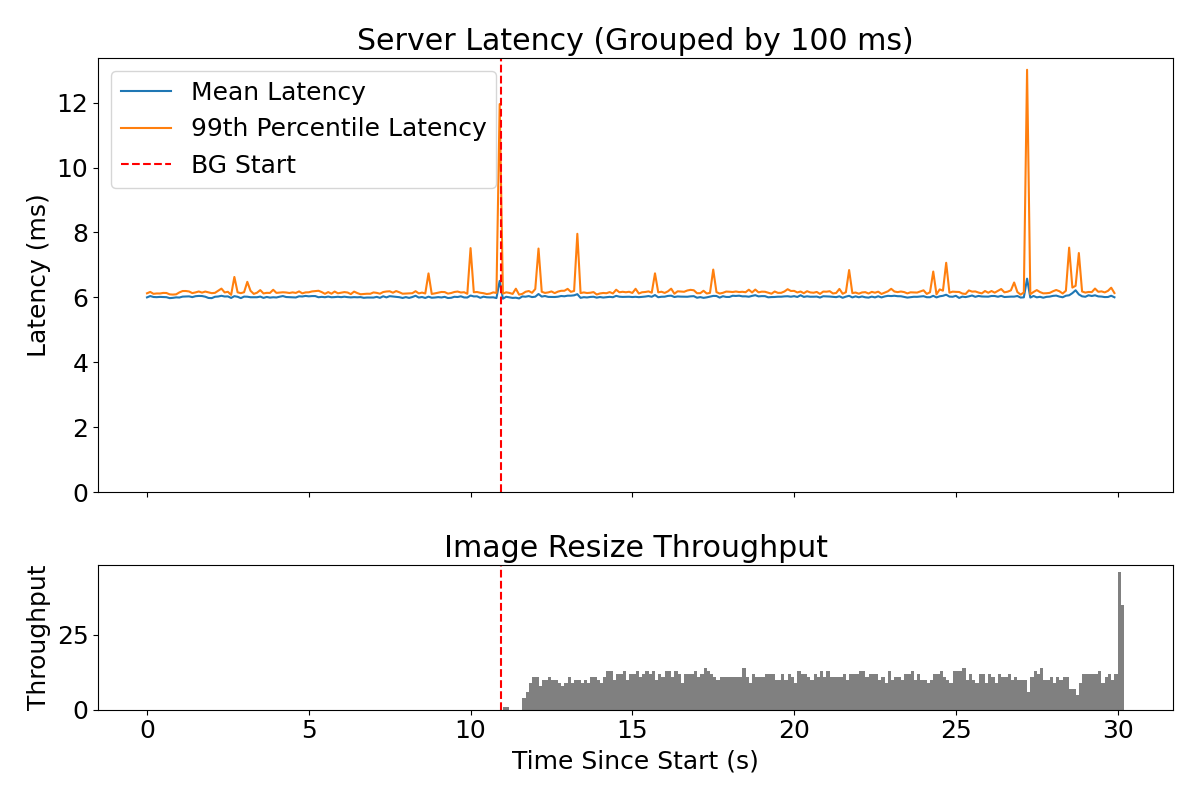
\includegraphics[width=\columnwidth]{graphs/srv-bg-schedbe-low.png}
        \caption{Low load (85\%)}\label{fig:srv-bg-schedbe-low}
        \vspace{12pt}
    \end{subfigure}
    \begin{subfigure}{\columnwidth}
        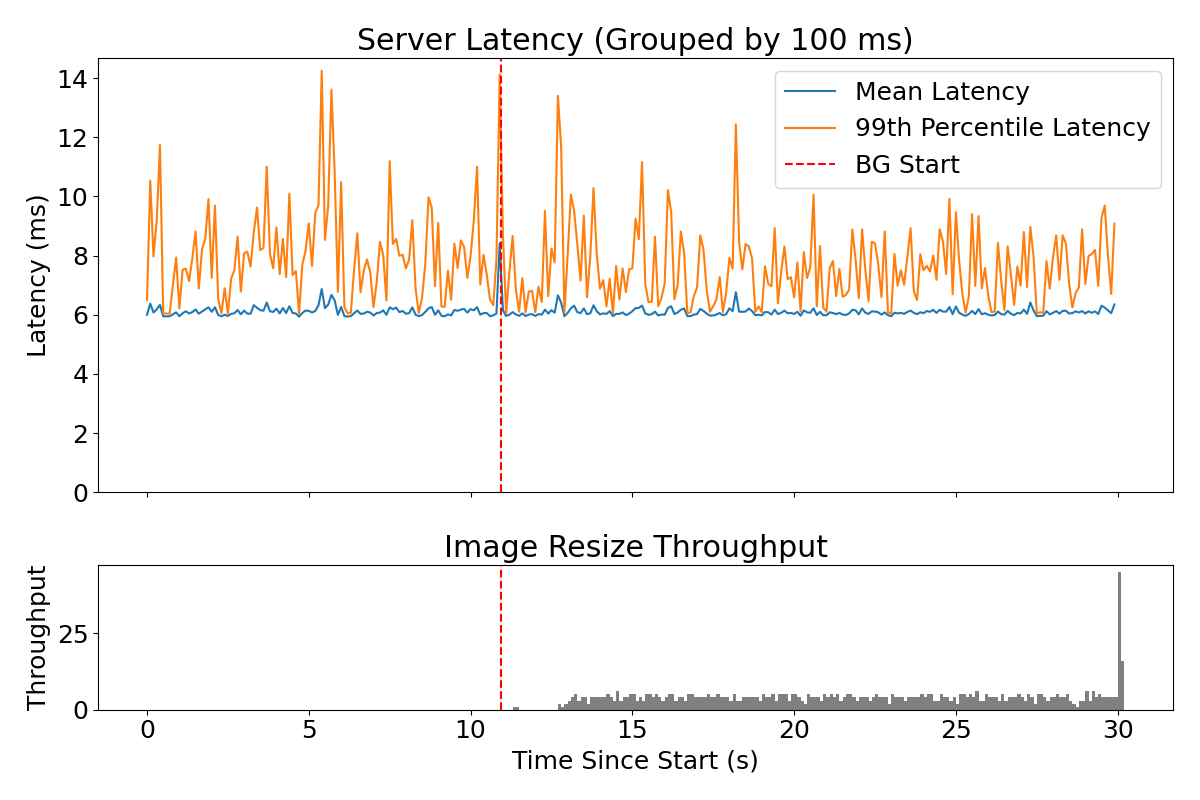
\includegraphics[width=\columnwidth]{graphs/srv-bg-schedbe-high.png}
        \caption{High load (95\%)}\label{fig:srv-bg-schedbe-high}
    \end{subfigure}
    \vspace{4pt}
    \caption{ \beclass{} does a good job of isolating the server's latencies
     from the load from best effort jobs}\label{fig:srv-bg-schedbe}
\end{figure}

\begin{figure}[t]
    \centering
    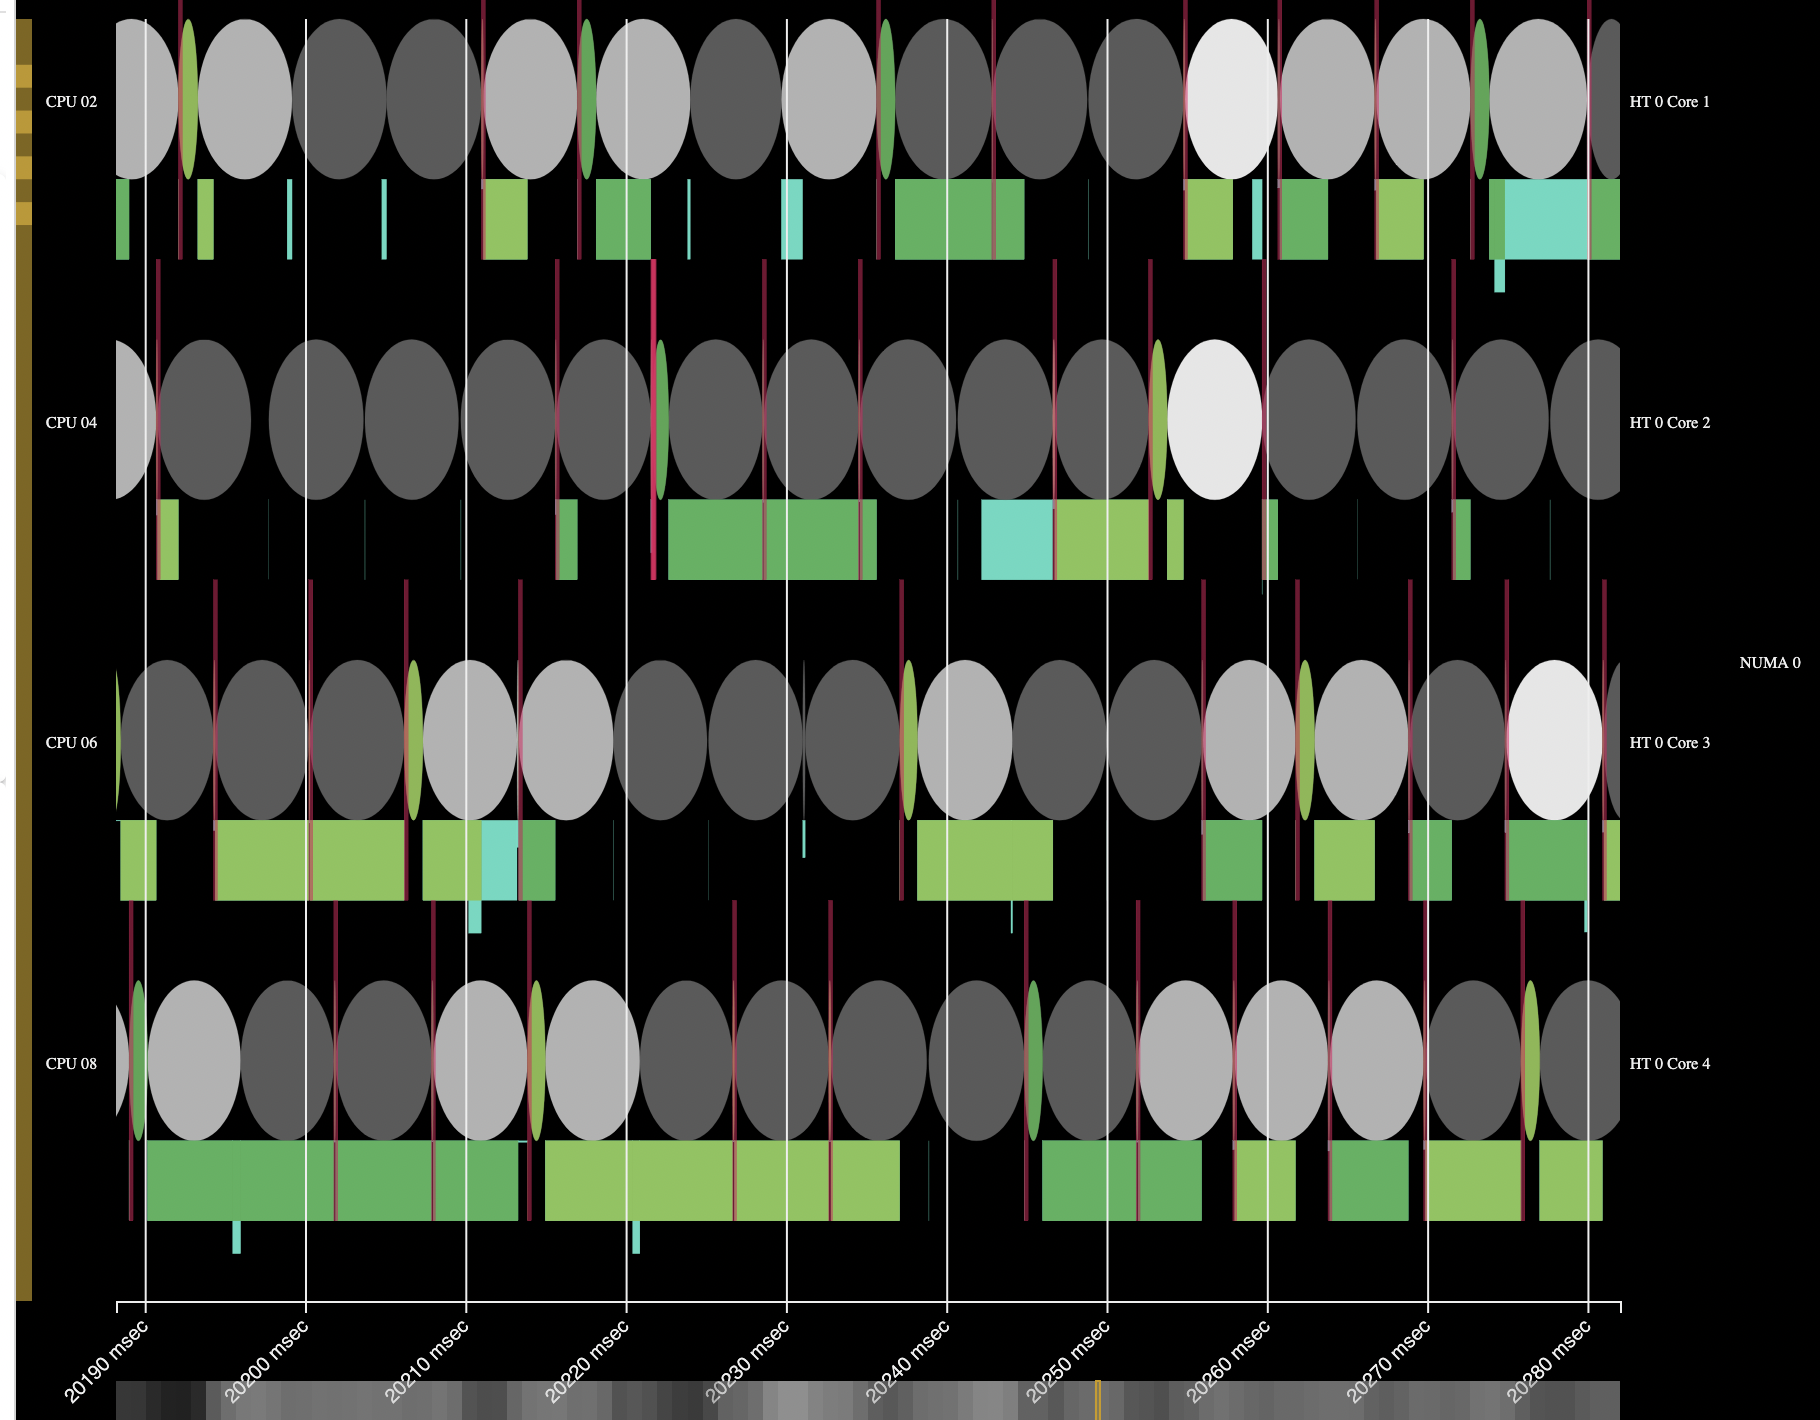
\includegraphics[width=\columnwidth]{graphs/schedviz-schedbe.png}
    \caption{BE threads only run in the gaps when there are no queued LC threads
    on any core }\label{fig:schedviz-schedbe}
\end{figure}

We run the microbenchmark experiment from \autoref{fig:srv-bg-weight-cmp} using
\beclass{}. We can see the resulting performance in
\autoref{fig:srv-bg-schedbe}. As desired, the latency of the server remains
stable after the background tasks start, and the background task still runs. 

Importantly, the background tasks will reliably get interrupted when the LC
server has a request to process. \autoref{fig:schedviz-schedbe} shows the
interruption happening in an outtake of a trace. The green BE processes run only
in the gaps where there is no queued LC process, and are immediately preempted
when one wakes up, on whatever core that may be. The vertical red lines show
when the \exit{} path \beclass{} introduced runs. As we can see, this line is
often followed by the core running an LC process, indicating it succesfully
found and stole a queued LC thread.

\begin{figure}[t]
    \centering
    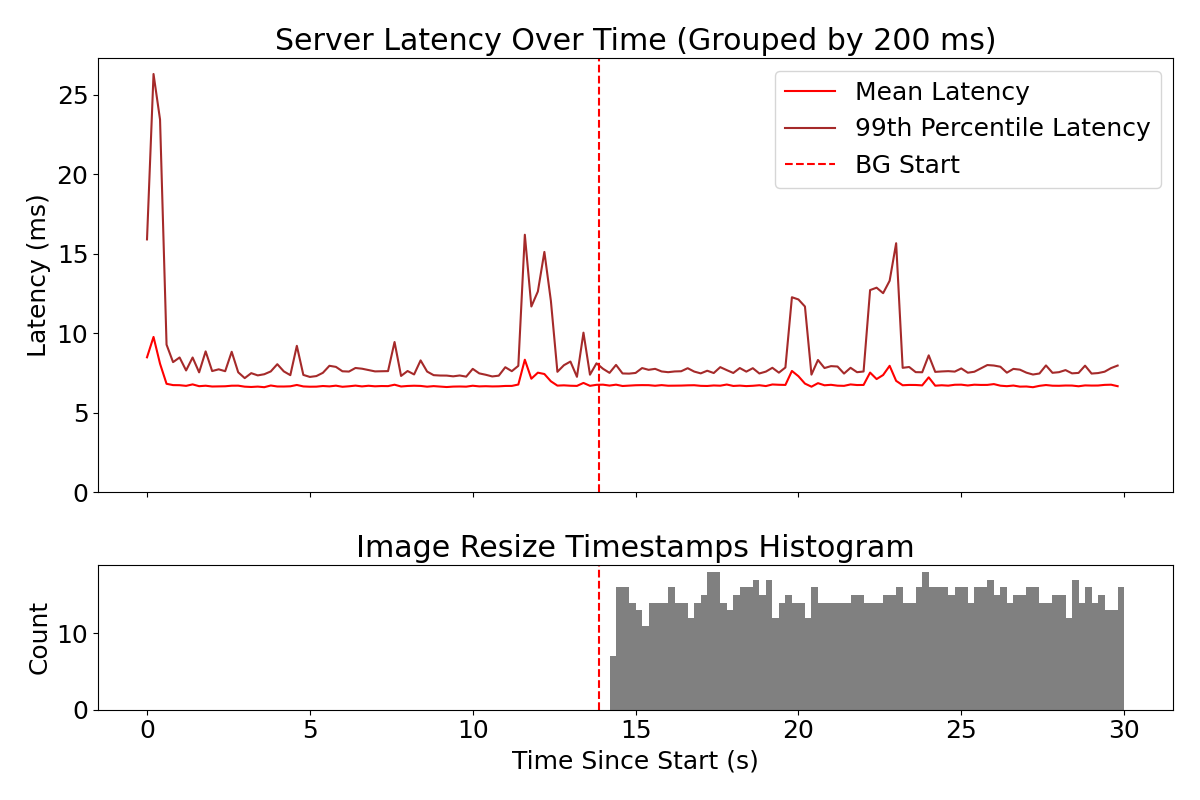
\includegraphics[width=\columnwidth]{graphs/kubernetes-schedbe.png}
    \caption{The same experiment as in \autoref{fig:kubernetes-unedited}, but
    running the BE as a \beclass{} task}\label{fig:kubernetes-schedbe}
\end{figure}

We also run the Kubernetes application from \autoref{fig:kubernetes-unedited}
using \beclass{}. The results are in \autoref{fig:kubernetes-schedbe}. We can
see that the baseline mean latency of the LC server stays around 7.4ms after
starting the the BE image resizing.